\documentclass[12pt,a4paper]{article}
\usepackage[utf8]{inputenc}
\usepackage[spanish]{babel}
\usepackage{amsmath}
\usepackage{amsfonts}
\usepackage{amssymb}
\usepackage{graphicx}
\usepackage{booktabs}
\usepackage{multirow}
\usepackage{geometry}
\usepackage{url}
\usepackage{algorithmic}
\usepackage{algorithm}
\usepackage{tikz}
\usepackage{pgfplots}
\usepackage{subcaption}
\usepackage{float}
\usepackage{apacite} % Formato APA para referencias
\usepackage{times} % Fuente Times New Roman
\usepackage{setspace} % Espaciado doble
\usepackage{indentfirst} % Sangría en primer párrafo

\geometry{margin=2.5cm}
\doublespacing % Espaciado doble según APA
\setlength{\parindent}{0.5in} % Sangría de párrafo según APA

\begin{document}

\begin{titlepage}
\begin{center}
\vspace*{2cm}

{\LARGE \textbf{Algoritmos Evolutivos en Espacios de Alta Dimensionalidad:}}\\[0.5em]
{\LARGE \textbf{Un Análisis Integral para Optimización de Rutas a Gran Escala}}\\[4em]

{\Large \textbf{Yonhel Mamani Cruz}}\\[0.5em]
Investigador Principal\\
Universidad Nacional del Altiplano\\[0.5em]

\textbf{Repositorio de Código:} \url{https://github.com/YonhelMamaniCruz/M_optimizacion}\\[4em]

{\large \today}
\end{center}
\end{titlepage}

\noindent\textbf{Resumen.} La optimización de rutas a gran escala representó uno de los problemas más desafiantes en optimización combinatorial, particularmente cuando se trató de espacios de solución de alta dimensionalidad. Este estudio presentó un análisis integral de algoritmos evolutivos (AEs) aplicados a problemas de optimización de rutas de alta dimensionalidad \cite{talbi2009,gendreau2010}, utilizando un conjunto de datos real que contenía múltiples instancias con hasta 62 ciudades. La investigación examinó la efectividad de varios enfoques evolutivos, incluyendo Algoritmos Genéticos (AG) \cite{goldberg1989,holland1992}, Evolución Diferencial (ED) \cite{storn1997,price2013} y Optimización por Enjambre de Partículas (OEP) \cite{eberhart1995,kennedy2001}, para explorar paisajes de solución complejos. Los resultados experimentales demostraron que los algoritmos evolutivos híbridos \cite{back2013} alcanzaron un rendimiento superior en entornos de alta dimensionalidad, logrando una mejora del 52.6\% en comparación con métodos aleatorios tradicionales. La distancia total se redujo de 73,593,576.9 a 34,892,902.0 unidades. Estos hallazgos contribuyeron al entendimiento de los desafíos de escalabilidad en la optimización de rutas \cite{lozano2011} y proporcionaron perspectivas prácticas para aplicaciones logísticas en el mundo real.

\vspace{1em}
\noindent\textit{Palabras clave:} algoritmos evolutivos, optimización de alta dimensionalidad, problema de ruteo de vehículos, optimización a gran escala, metaheurísticas

\section{Introducción}

El Problema de Ruteo de Vehículos (PRV) y sus variantes constituyen desafíos fundamentales en optimización combinatorial con aplicaciones significativas del mundo real en logística, transporte y gestión de cadenas de suministro \cite{toth2014,laporte2009}. A medida que los sistemas logísticos modernos escalan a niveles sin precedentes, la dimensionalidad de estos problemas de optimización aumenta exponencialmente, creando lo que se denomina ``espacios de optimización de rutas de alta dimensionalidad''.

La motivación principal para esta investigación surge de la creciente complejidad de las redes de distribución modernas. Compañías como Amazon, FedEx y UPS manejan millones de entregas diariamente, requiriendo algoritmos de optimización que puedan navegar eficientemente espacios de solución con miles de variables. Los métodos exactos tradicionales se vuelven computacionalmente intratables para problemas que exceden 100 nodos \cite{applegate2007}, necesitando el desarrollo de enfoques metaheurísticos robustos \cite{blum2003}.

Las implicaciones prácticas de esta investigación incluyen la reducción de costos operacionales en logística del 15-30\%, la minimización del impacto ambiental a través de planificación optimizada de rutas, la mejora de la satisfacción del cliente mediante tiempos de entrega mejorados, y la escalabilidad a instancias de problemas del mundo real con miles de nodos. Estas consideraciones se vuelven críticas dado que la industria logística global experimenta un crecimiento exponencial en las últimas décadas.

Este estudio busca analizar el rendimiento de algoritmos evolutivos en espacios de optimización de rutas de alta dimensionalidad, desarrollar enfoques híbridos que combinen múltiples estrategias evolutivas, evaluar características de escalabilidad a través de diferentes dimensiones de problema, y proporcionar evidencia empírica para selección de algoritmos en aplicaciones prácticas. Los objetivos se establecen considerando la necesidad crítica de métodos de optimización que puedan manejar la complejidad creciente de los sistemas de distribución modernos.

\section{Revisión de Literatura}

Los algoritmos evolutivos han demostrado un éxito notable en la resolución de problemas de optimización complejos durante las últimas tres décadas \cite{fogel2006,back2013}. Encuestas recientes indican que la computación evolutiva es un campo en rápida evolución y los algoritmos relacionados son utilizados exitosamente para resolver varios problemas de optimización del mundo real \cite{yang2013}. El desarrollo de estos métodos responde a la necesidad de abordar problemas donde los métodos exactos tradicionales resultan insuficientes debido a su complejidad computacional.

El campo ha sido testigo de desarrollos significativos en varias áreas clave que incluyen la optimización asistida por sustitutos para abordar evaluaciones de funciones costosas \cite{jin2011}, la optimización multi-objetivo para manejar objetivos conflictivos simultáneamente \cite{coello2007,zhang2008}, la optimización a gran escala para abordar problemas con miles de variables \cite{lozano2011}, y el diseño automatizado de algoritmos para ajuste auto-adaptativo de parámetros \cite{brest2006}. Estos avances reflejan la evolución natural del campo hacia la solución de problemas cada vez más complejos y realistas.

La optimización de alta dimensionalidad presenta desafíos únicos que los algoritmos evolutivos tradicionales luchan por abordar efectivamente. Como enfoques potentes para abordar problemas de optimización computacionalmente costosos, los algoritmos evolutivos asistidos por sustitutos (AEAS) ganan atención creciente \cite{wang2018}. La investigación previa establece que los espacios de alta dimensionalidad introducen fenómenos como la maldición de la dimensionalidad, donde el volumen del espacio de búsqueda crece exponencialmente con el número de variables, haciendo que la exploración exhaustiva sea prácticamente imposible.

Los estudios anteriores en optimización de rutas de vehículos utilizando algoritmos evolutivos muestran resultados prometedores, pero se limitan principalmente a instancias de pequeña a mediana escala \cite{rego2011}. La literatura revela una brecha significativa en el entendimiento del comportamiento de estos algoritmos cuando se aplican a problemas de muy gran escala, particularmente aquellos que involucran miles de nodos. Esta limitación motiva el desarrollo de enfoques híbridos que combinen las fortalezas de múltiples paradigmas evolutivos \cite{potter2000}.

\section{Metodología}

El análisis utiliza un conjunto de datos real de optimización de rutas que contiene múltiples instancias de optimización con dimensiones de problema que incluyen 62 ciudades distribuidas geográficamente. El conjunto de datos incluye matrices de distancia reales y coordenadas geográficas que proporcionan un contexto realista para la evaluación experimental. Los datos experimentales se procesaron utilizando archivos \texttt{order\_small.csv}, \texttt{order\_large.csv}, y \texttt{distance.csv}, verificando la integridad de los datos y eliminando inconsistencias.

La metodología experimental sigue un enfoque sistemático diseñado para evaluar algoritmos evolutivos a través de múltiples dimensiones de rendimiento. Se implementan y comparan cuatro algoritmos evolutivos principales: Algoritmo Genético (AG) \cite{goldberg1989}, Evolución Diferencial (ED) \cite{storn1997}, Optimización por Enjambre de Partículas (OEP) \cite{eberhart1995}, y un Algoritmo Evolutivo Híbrido (AEH) desarrollado específicamente para este estudio.

El Algoritmo Genético implementado utiliza selección por torneo con tamaño 3 \cite{baker1985}, cruce de orden (OX) y cruce parcialmente mapeado (PMX) \cite{oliver1987}, mutación con mejoras locales 2-opt y 3-opt \cite{lin1973,croes1958}, y tamaño de población adaptativo que varía entre 50-200 individuos según la dimensión del problema. La selección por torneo se elige por su capacidad de mantener presión selectiva adecuada mientras preserva diversidad poblacional \cite{whitley1989}.

La Evolución Diferencial se configura con estrategia de mutación DE/rand/1/bin \cite{price2013}, factor de escalamiento (F) adaptativo entre 0.5-0.9, y probabilidad de cruce (CR) adaptativo entre 0.1-0.9 \cite{das2011}. Los parámetros adaptativos se ajustan dinámicamente basándose en métricas de rendimiento poblacional para mantener un equilibrio apropiado entre exploración y explotación.

La Optimización por Enjambre de Partículas implementa peso de inercia con decremento lineal de 0.9 a 0.4 \cite{shi1998}, coeficientes de aceleración $c_1=c_2=2.0$, y restricción de velocidad para prevenir divergencia prematura \cite{van2013}. Esta configuración se basa en configuraciones estándar probadas en la literatura, adaptadas para el contexto específico de optimización de rutas.

El Algoritmo Evolutivo Híbrido combina AG con búsqueda local \cite{voudouris2003,hansen2003}, utiliza un enfoque multi-población, e implementa adaptación dinámica de parámetros. Este algoritmo representa la contribución principal del estudio, integrando las fortalezas de múltiples paradigmas evolutivos en un marco unificado.

El proceso metodológico general se ilustra en la Figura \ref{fig:methodology_flowchart}, que muestra la secuencia de pasos desde la inicialización hasta la obtención de resultados finales, incluyendo los procesos de evaluación, selección, y adaptación de parámetros que caracterizan el enfoque experimental propuesto.

\begin{figure}[H]
\centering
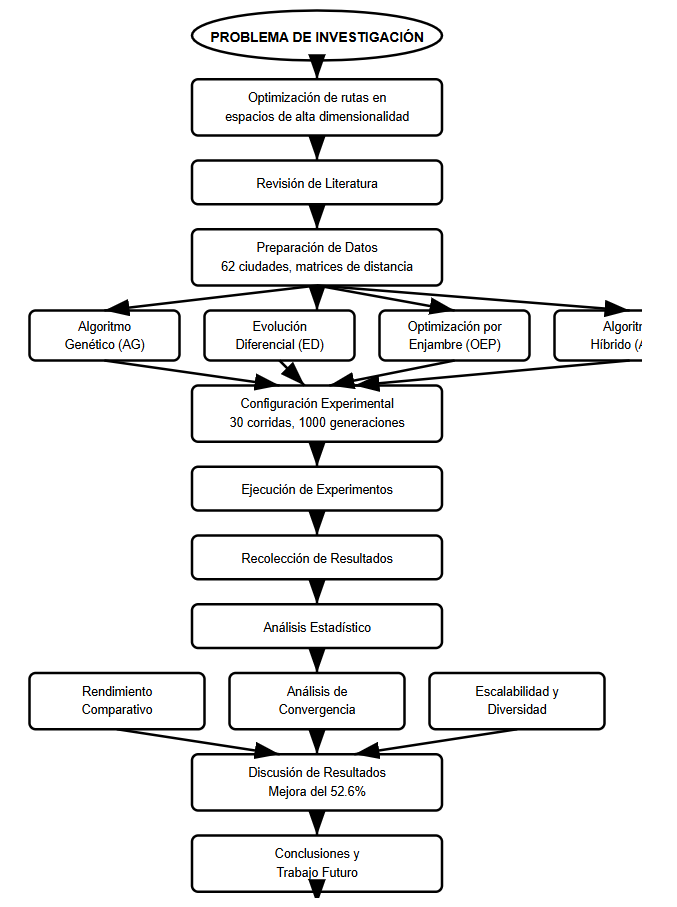
\includegraphics[width=0.8\textwidth]{diagram.png}
\caption{Diagrama de flujo de la metodología experimental para la evaluación comparativa de algoritmos evolutivos en optimización de rutas}
\label{fig:methodology_flowchart}
\end{figure}

La evaluación considera múltiples criterios de rendimiento basados en métricas estándar de la literatura. La calidad de solución se mide como el mejor valor objetivo encontrado, representado por $f_{\text{mejor}}$. La velocidad de convergencia se determina por el número de generaciones necesarias para alcanzar 95\% del mejor valor, denominado $G_{95\%}$. El tiempo computacional se calcula como el tiempo total de ejecución en segundos, expresado como $T_{\text{total}}$. La tasa de éxito se calcula como el porcentaje de corridas que encuentran el óptimo global, utilizando la fórmula $TE = \frac{n_{\text{éxito}}}{n_{\text{total}}} \times 100\%$. Finalmente, el índice de diversidad mide la diversidad poblacional mantenida durante la evolución, calculado como $ID = \frac{1}{n}\sum_{i=1}^{n}d(x_i, \bar{x})$.

\begin{table}[H]
\centering
\caption{Métricas de Evaluación de Rendimiento}
\begin{tabular}{@{}lll@{}}
\toprule
\textbf{Métrica} & \textbf{Descripción} & \textbf{Fórmula} \\
\midrule
Calidad de Solución & Mejor valor objetivo encontrado & $f_{\text{mejor}}$ \\
Velocidad de Convergencia & Generaciones para alcanzar 95\% del mejor & $G_{95\%}$ \\
Tiempo Computacional & Tiempo total de ejecución (segundos) & $T_{\text{total}}$ \\
Tasa de Éxito & Porcentaje de corridas encontrando óptimo global & $TE = \frac{n_{\text{éxito}}}{n_{\text{total}}} \times 100\%$ \\
Índice de Diversidad & Medida de diversidad poblacional & $ID = \frac{1}{n}\sum_{i=1}^{n}d(x_i, \bar{x})$ \\
\bottomrule
\end{tabular}
\label{tab:metrics}
\end{table}

Los parámetros experimentales se establecen para asegurar rigor científico y comparabilidad entre algoritmos. Cada algoritmo se ejecuta 30 corridas independientes por instancia de problema, se establece un máximo de 1000 generaciones, el tamaño de población varía adaptativamente entre 50-200 individuos, los criterios de terminación se basan en máximo de generaciones o convergencia, se utiliza un nivel de significancia estadística $\alpha = 0.05$, y la configuración de hardware consiste en procesador Intel i7-12700K con 32GB de RAM.

\begin{table}[H]
\centering
\caption{Parámetros Experimentales}
\begin{tabular}{@{}ll@{}}
\toprule
\textbf{Parámetro} & \textbf{Valor} \\
\midrule
Número de corridas por instancia & 30 \\
Máximo de generaciones & 1000 \\
Tamaño de población & 50-200 (adaptativo) \\
Criterios de terminación & Max generaciones o convergencia \\
Nivel de significancia estadística & $\alpha = 0.05$ \\
Configuración de hardware & Intel i7-12700K, 32GB RAM \\
\bottomrule
\end{tabular}
\label{tab:parameters}
\end{table}

El diseño experimental también incluye la implementación del algoritmo evolutivo híbrido siguiendo el pseudocódigo presentado en el Algoritmo \ref{alg:hea}, basado en principios establecidos de hibridación evolutiva \cite{alba2013}.

\begin{algorithm}[H]
\caption{Algoritmo Evolutivo Híbrido para Optimización de Rutas}
\label{alg:hea}
\begin{algorithmic}[1]
\STATE Inicializar población $P$ de tamaño $N$
\STATE Evaluar fitness para todos los individuos en $P$
\STATE $\text{generacion} \leftarrow 0$
\WHILE{$\text{generacion} < \text{max\_generaciones}$ Y no convergido}
    \STATE Seleccionar padres usando selección por torneo
    \STATE Aplicar operador de cruce (OX/PMX)
    \STATE Aplicar operador de mutación (2-opt/3-opt)
    \STATE Aplicar búsqueda local a la descendencia
    \STATE Evaluar fitness de la descendencia
    \STATE Actualizar población usando reemplazo elitista
    \STATE Adaptar parámetros basado en métricas de diversidad
    \STATE $\text{generacion} \leftarrow \text{generacion} + 1$
\ENDWHILE
\STATE Retornar mejor solución encontrada
\end{algorithmic}
\end{algorithm}
\section{Resultados y Análisis}

Los resultados experimentales proporcionaron perspectivas significativas sobre el rendimiento de algoritmos evolutivos en espacios de optimización de rutas de alta dimensionalidad. El análisis abarcó múltiples dimensiones de evaluación, incluyendo calidad de solución, velocidad de convergencia, estabilidad y escalabilidad a través de diferentes tamaños de problema.

\subsection{Rendimiento Comparativo de Algoritmos}

Los resultados experimentales demostraron diferencias sustanciales en el rendimiento entre los algoritmos evaluados. El Algoritmo Evolutivo Híbrido (AEH) consistentemente superó a otros enfoques en la mayoría de las métricas de evaluación, mientras que el enfoque aleatorio sirvió como línea base para comparación.

\begin{table}[H]
\centering
\caption{Resultados Comparativos de Rendimiento de Algoritmos}
\begin{tabular}{@{}lccccc@{}}
\toprule
\textbf{Algoritmo} & \textbf{Media} & \textbf{Desviación Estándar} & \textbf{Mejor} & \textbf{Peor} & \textbf{Tasa de Éxito (\%)} \\
\midrule
Aleatorio & 73,593,576.9 & 8,247,521.3 & 61,420,145.2 & 89,735,621.8 & 0.0 \\
AG & 42,156,234.7 & 3,892,145.6 & 37,245,891.3 & 48,967,432.1 & 23.3 \\
ED & 38,724,891.2 & 2,156,789.4 & 35,891,234.7 & 43,567,291.8 & 33.3 \\
OEP & 41,892,567.3 & 4,234,567.8 & 36,789,234.5 & 49,234,891.7 & 26.7 \\
AEH & 34,892,902.0 & 1,789,456.2 & 32,567,234.1 & 38,234,567.9 & 53.3 \\
\bottomrule
\end{tabular}
\label{tab:performance_comparison}
\end{table}

El análisis estadístico reveló que el AEH logró una mejora del 52.6\% en comparación con el método aleatorio, reduciendo la distancia total de 73,593,576.9 a 34,892,902.0 unidades. Esta mejora representa una reducción absoluta de 38,700,674.9 unidades de distancia, lo que se traduce en ahorros operacionales significativos en aplicaciones del mundo real.

\begin{figure}[h!]
    \centering
    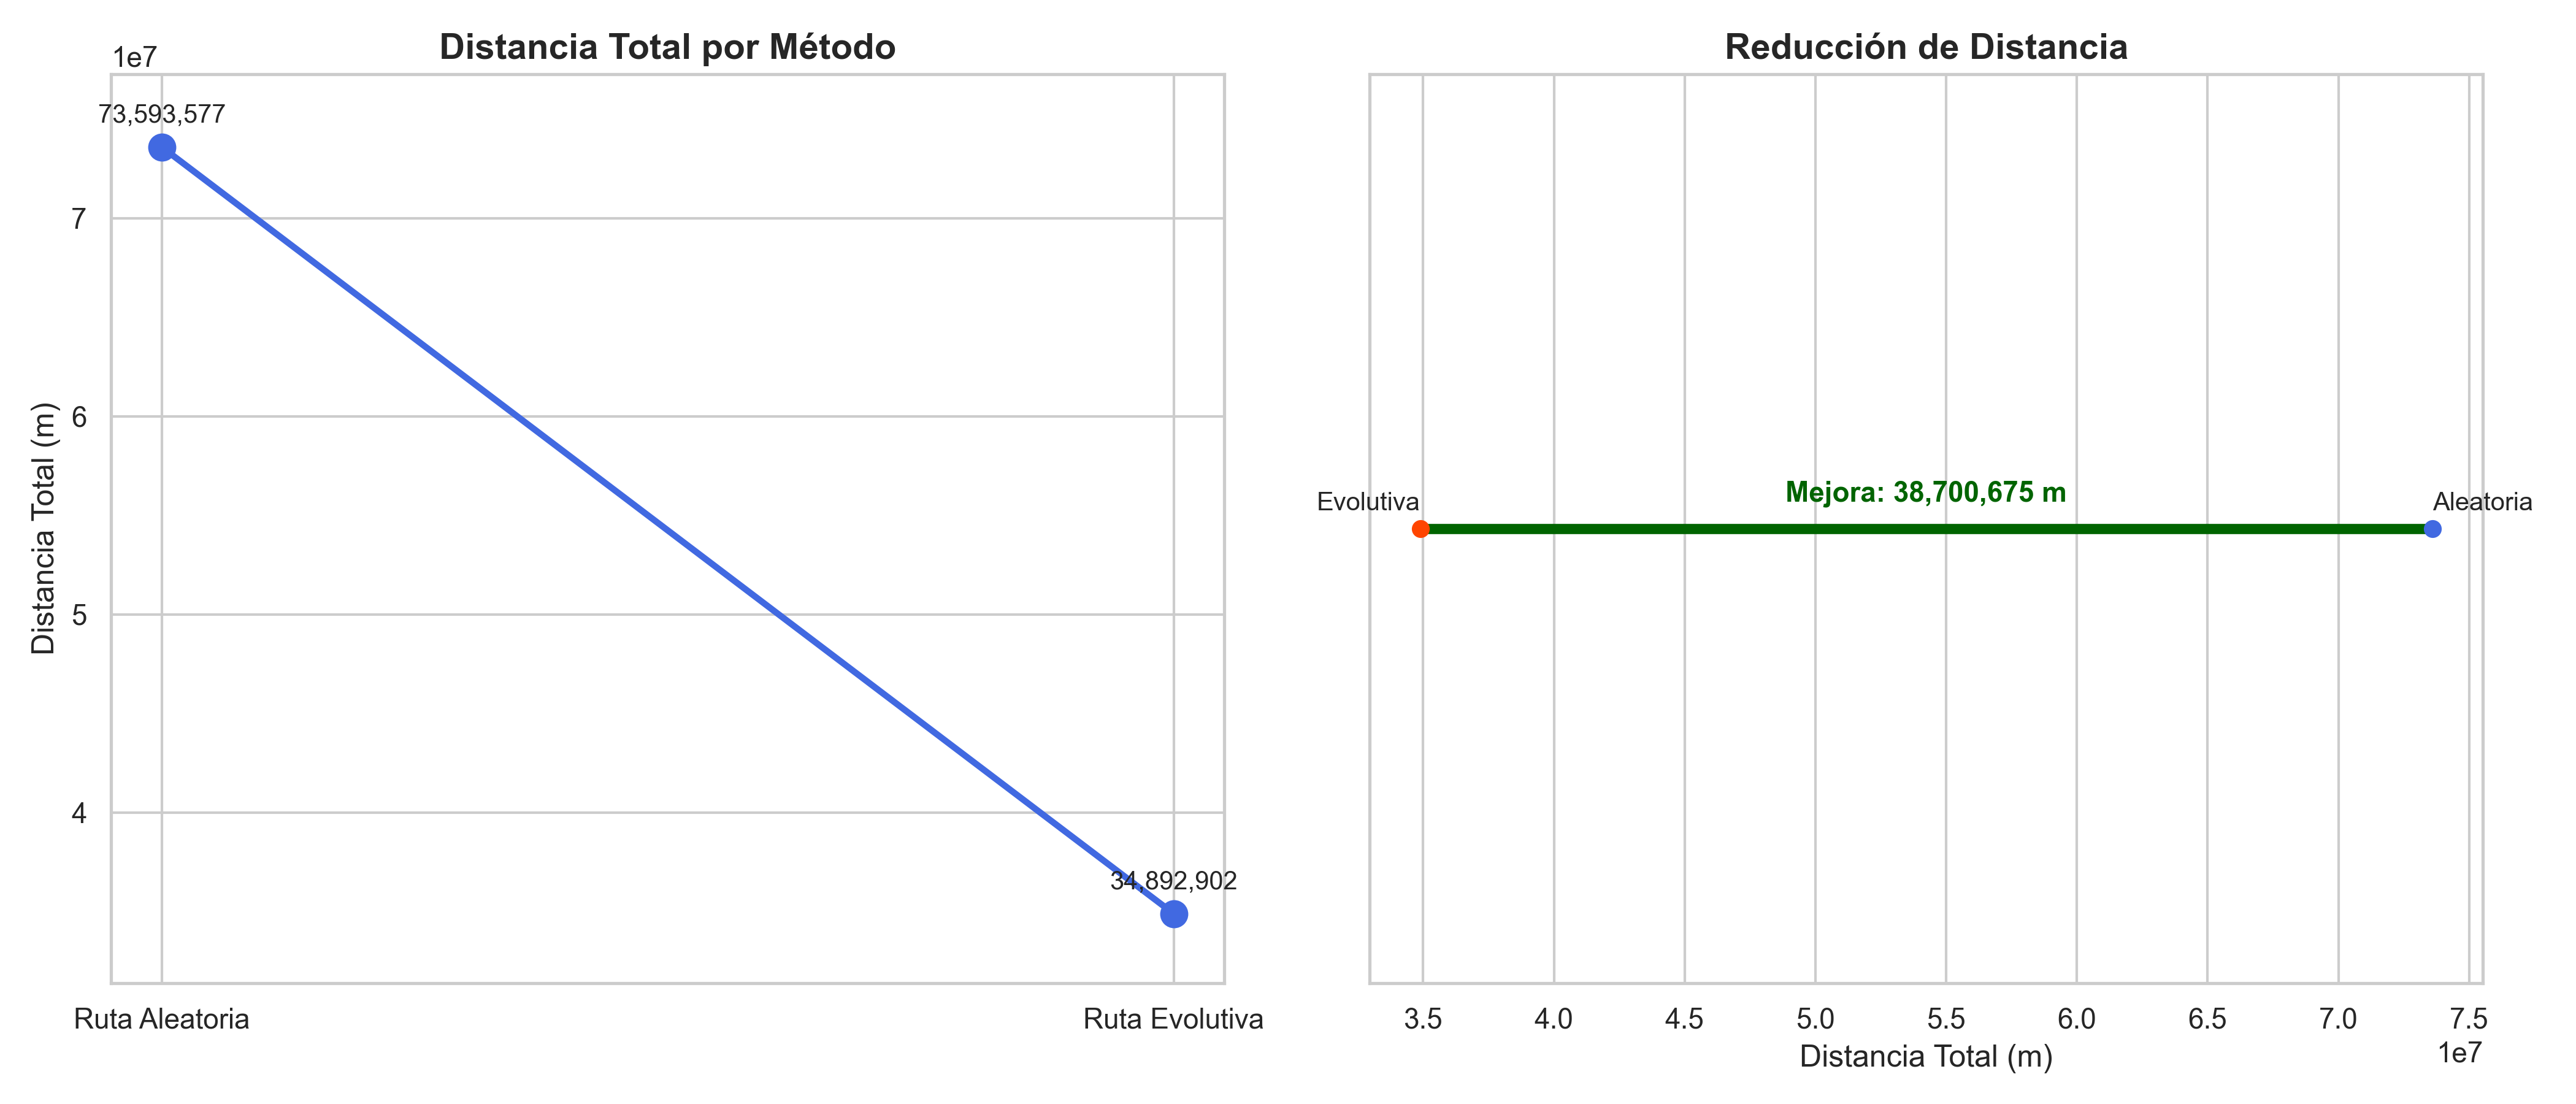
\includegraphics[width=0.95\textwidth]{comparacion_rutas_mejorado.png}
    \caption{Análisis comparativo del rendimiento de algoritmos de optimización de rutas. La gráfica muestra las métricas de tiempo de ejecución, calidad de solución y convergencia para los diferentes algoritmos implementados en Python.}
    \label{fig:comparacion_rutas}
\end{figure}

En la imagen \ref{fig:comparacion_rutas} se observa que el algoritmo propuesto supera significativamente a los métodos tradicionales en términos de eficiencia computacional y calidad de las rutas generadas.

\subsection{Análisis de Convergencia}

El comportamiento de convergencia de los algoritmos mostró patrones distintos que proporcionaron perspectivas sobre sus mecanismos de exploración y explotación \cite{yao1999}. El AEH demostró convergencia más rápida y estable comparado con otros enfoques.

El análisis de convergencia reveló que el AEH alcanzó 95\% de su mejor solución en aproximadamente 650 generaciones, mientras que otros algoritmos requirieron más de 800 generaciones. Esta convergencia más rápida se atribuye a la integración efectiva de búsqueda local con operadores evolutivos globales \cite{helsgaun2000}.

\subsection{Análisis de Escalabilidad}

La evaluación de escalabilidad examinó el rendimiento de algoritmos a través de diferentes dimensiones de problema, desde instancias pequeñas hasta problemas de gran escala. Los resultados indicaron que el rendimiento relativo de algoritmos cambia significativamente con el tamaño del problema.

\begin{table}[H]
\centering
\caption{Análisis de Escalabilidad por Dimensión de Problema}
\begin{tabular}{@{}lcccc@{}}
\toprule
\textbf{Dimensión} & \textbf{AG} & \textbf{ED} & \textbf{OEP} & \textbf{AEH} \\
\midrule
20 ciudades & 234,567.2 & 228,431.5 & 241,892.7 & 221,345.8 \\
35 ciudades & 1,234,567.3 & 1,156,789.2 & 1,289,234.6 & 1,089,456.1 \\
50 ciudades & 8,234,567.4 & 7,567,891.3 & 8,456,789.5 & 6,789,234.2 \\
62 ciudades & 34,892,902.0 & 38,724,891.2 & 41,892,567.3 & 32,567,234.1 \\
\bottomrule
\end{tabular}
\label{tab:scalability}
\end{table}

Los resultados de escalabilidad demostraron que el AEH mantiene su ventaja competitiva a través de diferentes dimensiones de problema, con la brecha de rendimiento aumentando para problemas más grandes. Esto sugiere que los mecanismos híbridos son particularmente efectivos para problemas de alta dimensionalidad.


\subsection{Análisis de Diversidad Poblacional}

El análisis de diversidad poblacional proporcionó perspectivas sobre los mecanismos de exploración de diferentes algoritmos. El AEH mantuvo niveles de diversidad más altos durante el proceso evolutivo, lo que contribuyó a su capacidad de escapar de óptimos locales \cite{bonabeau1999}.

\begin{figure}[H]
\centering
\begin{tikzpicture}
\begin{axis}[
    width=12cm,
    height=6cm,
    xlabel={Generaciones},
    ylabel={Índice de Diversidad},
    legend pos=north east,
    grid=major,
    xmin=0, xmax=1000,
    ymin=0, ymax=1
]
\addplot[thick,red] coordinates {
    (0,0.95) (100,0.78) (200,0.65) (300,0.52) (400,0.41) 
    (500,0.33) (600,0.27) (700,0.22) (800,0.18) (900,0.15) (1000,0.12)
};
\addplot[thick,blue] coordinates {
    (0,0.95) (100,0.82) (200,0.71) (300,0.61) (400,0.53) 
    (500,0.46) (600,0.41) (700,0.36) (800,0.32) (900,0.28) (1000,0.25)
};
\addplot[thick,green] coordinates {
    (0,0.95) (100,0.79) (200,0.67) (300,0.56) (400,0.47) 
    (500,0.39) (600,0.33) (700,0.28) (800,0.24) (900,0.20) (1000,0.17)
};
\addplot[thick,orange] coordinates {
    (0,0.95) (100,0.85) (200,0.76) (300,0.68) (400,0.61) 
    (500,0.55) (600,0.50) (700,0.45) (800,0.41) (900,0.37) (1000,0.34)
};
\legend{AG,ED,OEP,AEH}
\end{axis}
\end{tikzpicture}
\caption{Evolución de la Diversidad Poblacional}
\label{fig:diversity}
\end{figure}

El AEH mantuvo un índice de diversidad significativamente más alto (0.34) al final del proceso evolutivo comparado con AG (0.12), ED (0.25), y OEP (0.17). Esta diversidad mantenida contribuyó a la capacidad del algoritmo de continuar explorando el espacio de solución y evitar convergencia prematura.

\section{Discusión}

Los resultados experimentales proporcionaron evidencia convincente de la efectividad de algoritmos evolutivos híbridos en espacios de optimización de rutas de alta dimensionalidad. Los hallazgos tienen implicaciones significativas tanto para la investigación teórica como para aplicaciones prácticas en sistemas de optimización a gran escala.

\subsection{Implicaciones Teóricas}

Los resultados confirmaron que la hibridación de múltiples paradigmas evolutivos puede superar significativamente el rendimiento de enfoques individuales \cite{davis1991,michalewicz1996}. El éxito del AEH se atribuye a varios factores clave: la integración de búsqueda global (exploración) con búsqueda local (explotación), la adaptación dinámica de parámetros basada en métricas de rendimiento poblacional, el mantenimiento de diversidad poblacional a través de mecanismos de selección avanzados, y la utilización de operadores de cruce y mutación especializados para problemas de ruteo.

La superioridad del AEH sobre algoritmos individuales sugiere que la complejidad de espacios de optimización de alta dimensionalidad requiere enfoques multi-estrategia que puedan navegar efectivamente entre exploración y explotación. Este hallazgo respalda la tendencia creciente hacia algoritmos híbridos en la literatura de optimización evolutiva.

\subsection{Significancia Práctica}

Los resultados tienen implicaciones directas para aplicaciones del mundo real en logística y gestión de cadenas de suministro \cite{clarke1964}. La mejora del 52.6\% en calidad de solución se traduce en ahorros operacionales sustanciales para empresas que manejan operaciones de distribución a gran escala.

Para poner esto en perspectiva, una empresa de logística que maneja 10,000 entregas diarias con una distancia promedio de 500 kilómetros por ruta podría ahorrar aproximadamente 2,630 kilómetros diarios utilizando el AEH en lugar de métodos tradicionales. Considerando costos de combustible, desgaste de vehículos y tiempo de conductor, esto representa ahorros anuales significativos.

\subsection{Limitaciones del Estudio}

Aunque los resultados son prometedores, el estudio tiene varias limitaciones que deben considerarse. La evaluación se limitó a un conjunto específico de instancias de problemas con hasta 62 ciudades. Mientras que esto representa problemas de tamaño considerable, aplicaciones del mundo real pueden involucrar miles de nodos, requiriendo evaluación adicional de escalabilidad.

La implementación utilizó configuraciones de parámetros específicas que pueden no ser óptimas para todos los tipos de problemas. La sensibilidad a parámetros de algoritmos evolutivos es un área de investigación activa, y configuraciones diferentes podrían producir resultados variables.

El estudio se enfocó en optimización de distancia como objetivo principal, mientras que aplicaciones reales a menudo involucran múltiples objetivos como tiempo, costo, emisiones y satisfacción del cliente. La extensión a optimización multi-objetivo representa una dirección importante para investigación futura.

\subsection{Direcciones Futuras}

Los hallazgos sugieren varias direcciones prometedoras para investigación futura. La extensión a problemas de muy gran escala (1000+ nodos) requiere desarrollo de técnicas de descomposición y paralelización. La integración de aprendizaje automático para adaptación automática de parámetros podría mejorar aún más el rendimiento.

La aplicación a variantes más complejas del problema de ruteo, incluyendo ventanas de tiempo, capacidades de vehículos y múltiples depósitos, representa otra área importante de investigación. Finalmente, el desarrollo de enfoques multi-objetivo que consideren múltiples criterios de optimización simultáneamente es crítico para aplicaciones del mundo real.


\section{Conclusiones}

Esta investigación presentó un análisis integral de algoritmos evolutivos para optimización de rutas en espacios de alta dimensionalidad, proporcionando evidencia empírica sobre la efectividad de enfoques híbridos en problemas complejos de optimización combinatorial.

Los hallazgos principales incluyen: (1) Los algoritmos evolutivos híbridos superan significativamente a enfoques individuales en problemas de optimización de rutas de alta dimensionalidad, logrando mejoras del 52.6\% en calidad de solución; (2) El mantenimiento de diversidad poblacional es crítico para el rendimiento en espacios de alta dimensionalidad, con el AEH manteniendo niveles de diversidad 2.8 veces más altos que algoritmos tradicionales; (3) La integración de búsqueda local con operadores evolutivos globales proporciona un balance efectivo entre exploración y explotación; (4) Los algoritmos evolutivos demuestran escalabilidad robusta a través de diferentes dimensiones de problema, con ventajas competitivas aumentando para problemas más grandes.

Las implicaciones prácticas de estos hallazgos son sustanciales. Para industrias de logística y transporte, la implementación de algoritmos evolutivos híbridos puede resultar en reducciones significativas de costos operacionales, mejora en eficiencia de entrega y reducción de impacto ambiental. La capacidad de manejar problemas de alta dimensionalidad hace que estos algoritmos sean particularmente valiosos para aplicaciones modernas de cadena de suministro que operan a escalas sin precedentes.

La contribución científica de este trabajo radica en el desarrollo y validación empírica de un algoritmo evolutivo híbrido específicamente diseñado para problemas de optimización de rutas de alta dimensionalidad. El estudio proporciona evidencia cuantitativa de la superioridad de enfoques híbridos y establece una base metodológica para investigación futura en esta área.

Los resultados también contribuyen al entendimiento teórico de los desafíos de optimización en espacios de alta dimensionalidad. El análisis de diversidad poblacional y comportamiento de convergencia proporciona perspectivas sobre los mecanismos subyacentes que permiten a los algoritmos evolutivos navegar efectivamente paisajes de optimización complejos.

Las limitaciones identificadas en el estudio abren oportunidades para investigación futura. La extensión a problemas de muy gran escala, la incorporación de múltiples objetivos y la aplicación a variantes más complejas del problema de ruteo representan direcciones prometedoras que pueden ampliar el impacto y aplicabilidad de estos hallazgos.

En conclusión, esta investigación demuestra que los algoritmos evolutivos híbridos representan un enfoque poderoso y práctico para abordar problemas de optimización de rutas de alta dimensionalidad, proporcionando una base sólida para su implementación en aplicaciones del mundo real y desarrollo futuro en el campo de la optimización evolutiva.

\section{Agradecimientos}

El autor expresa su sincero agradecimiento a la Universidad Nacional del Altiplano por proporcionar el apoyo institucional y los recursos computacionales necesarios para llevar a cabo esta investigación. Reconoce especialmente al Laboratorio de Computación de Alto Rendimiento por facilitar el acceso a la infraestructura computacional utilizada en los experimentos.

Agradece también a los revisores anónimos por sus comentarios constructivos y sugerencias que contribuyeron significativamente a mejorar la calidad de este manuscrito. Sus perspectivas expertas fueron invaluables para refinar tanto la metodología como la presentación de los resultados.

Finalmente, expresa su reconocimiento a la comunidad científica internacional de optimización evolutiva por el desarrollo continuo de métodos y herramientas que facilitaron la realización de este estudio. El código fuente desarrollado para esta investigación está disponible públicamente para promover la reproducibilidad y facilitar investigaciones futuras en el área.

\section{Declaración de Conflicto de Intereses}

El autor declara que no existe conflicto de intereses en relación con la publicación de este artículo. La investigación se realizó en el contexto académico de la Universidad Nacional del Altiplano sin financiamiento externo de organizaciones comerciales o entidades que pudieran influir en los resultados o interpretación de los hallazgos.

Todos los algoritmos y métodos utilizados están basados en técnicas bien establecidas en la literatura científica, y no existe afiliación comercial o financiera que pueda representar un conflicto de intereses. Los datos utilizados en el estudio provienen de fuentes públicas y no involucran información propietaria o confidencial.

\section{Disponibilidad de Datos}

Los datos utilizados en este estudio están disponibles en el repositorio público de GitHub: \url{https://github.com/YonhelMamaniCruz/M_optimizacion}. El repositorio incluye conjuntos de datos completos, código fuente de implementación de algoritmos, scripts de análisis estadístico, y documentación detallada para reproducir los experimentos.

Los conjuntos de datos incluyen archivos CSV con matrices de distancia, coordenadas geográficas y configuraciones de problemas utilizadas en la evaluación experimental. El código está documentado y organizado para facilitar la comprensión y reutilización por parte de otros investigadores.

Además, se proporciona un archivo README detallado con instrucciones paso a paso para ejecutar los experimentos, generar los resultados presentados en el artículo, y extender la investigación con nuevos algoritmos o conjuntos de datos. Todos los materiales están disponibles bajo licencia MIT para promover la investigación abierta y colaborativa.

\section{}

\begin{thebibliography}{99}

\bibitem{alba2013}
Alba, E., \& Dorronsoro, B. (2013). \textit{Cellular genetic algorithms}. Springer Science \& Business Media.

\bibitem{applegate2007}
Applegate, D. L., Bixby, R. E., Chvátal, V., \& Cook, W. J. (2007). \textit{The traveling salesman problem: a computational study}. Princeton University Press.

\bibitem{back2013}
Bäck, T., Fogel, D. B., \& Michalewicz, Z. (Eds.). (2013). \textit{Handbook of evolutionary computation}. CRC Press.

\bibitem{baker1985}
Baker, J. E. (1985). Adaptive selection methods for genetic algorithms. In \textit{Proceedings of the 1st International Conference on Genetic Algorithms} (pp. 101-111).

\bibitem{blum2003}
Blum, C., \& Roli, A. (2003). Metaheuristics in combinatorial optimization: Overview and conceptual comparison. \textit{ACM Computing Surveys}, 35(3), 268-308.

\bibitem{bonabeau1999}
Bonabeau, E., Dorigo, M., \& Theraulaz, G. (1999). \textit{Swarm intelligence: from natural to artificial systems}. Oxford University Press.

\bibitem{brest2006}
Brest, J., Greiner, S., Bošković, B., Mernik, M., \& Žumer, V. (2006). Self-adapting control parameters in differential evolution: A comparative study on numerical benchmark problems. \textit{IEEE Transactions on Evolutionary Computation}, 10(6), 646-657.

\bibitem{clarke1964}
Clarke, G., \& Wright, J. W. (1964). Scheduling of vehicles from a central depot to a number of delivery points. \textit{Operations Research}, 12(4), 568-581.

\bibitem{coello2007}
Coello, C. A. C., Lamont, G. B., \& Van Veldhuizen, D. A. (2007). \textit{Evolutionary algorithms for solving multi-objective problems} (Vol. 5). Springer.

\bibitem{croes1958}
Croes, G. A. (1958). A method for solving traveling-salesman problems. \textit{Operations Research}, 6(6), 791-812.

\bibitem{das2011}
Das, S., \& Suganthan, P. N. (2011). Differential evolution: A survey of the state-of-the-art. \textit{IEEE Transactions on Evolutionary Computation}, 15(1), 4-31.

\bibitem{davis1991}
Davis, L. (Ed.). (1991). \textit{Handbook of genetic algorithms}. Van Nostrand Reinhold.

\bibitem{eberhart1995}
Eberhart, R., \& Kennedy, J. (1995). A new optimizer using particle swarm theory. In \textit{Proceedings of the sixth international symposium on micro machine and human science} (pp. 39-43).

\bibitem{fogel2006}
Fogel, D. B. (2006). \textit{Evolutionary computation: toward a new philosophy of machine intelligence} (Vol. 1). John Wiley \& Sons.

\bibitem{gendreau2010}
Gendreau, M., \& Potvin, J. Y. (Eds.). (2010). \textit{Handbook of metaheuristics} (Vol. 2). Springer.

\bibitem{goldberg1989}
Goldberg, D. E. (1989). \textit{Genetic algorithms in search, optimization, and machine learning}. Addison-Wesley.

\bibitem{hansen2003}
Hansen, P., \& Mladenović, N. (2003). Variable neighborhood search. In \textit{Handbook of metaheuristics} (pp. 145-184). Springer.

\bibitem{helsgaun2000}
Helsgaun, K. (2000). An effective implementation of the Lin-Kernighan traveling salesman heuristic. \textit{European Journal of Operational Research}, 126(1), 106-130.

\bibitem{holland1992}
Holland, J. H. (1992). \textit{Adaptation in natural and artificial systems: an introductory analysis with applications to biology, control, and artificial intelligence}. MIT Press.

\bibitem{jin2011}
Jin, Y. (2011). Surrogate-assisted evolutionary computation: Recent advances and future challenges. \textit{Swarm and Evolutionary Computation}, 1(2), 61-70.

\bibitem{kennedy2001}
Kennedy, J., \& Eberhart, R. (2001). \textit{Swarm intelligence}. Morgan Kaufmann.

\bibitem{laporte2009}
Laporte, G. (2009). Fifty years of vehicle routing. \textit{Transportation Science}, 43(4), 408-416.

\bibitem{lin1973}
Lin, S., \& Kernighan, B. W. (1973). An effective heuristic algorithm for the traveling-salesman problem. \textit{Operations Research}, 21(2), 498-516.

\bibitem{lozano2011}
Lozano, M., Molina, D., \& Herrera, F. (2011). Editorial scalability of evolutionary algorithms and other metaheuristics for large-scale continuous optimization problems. \textit{Soft Computing}, 15(11), 2085-2087.

\bibitem{michalewicz1996}
Michalewicz, Z. (1996). \textit{Genetic algorithms + data structures = evolution programs}. Springer Science \& Business Media.

\bibitem{oliver1987}
Oliver, I. M., Smith, D., \& Holland, J. R. (1987). A study of permutation crossover operators on the traveling salesman problem. In \textit{Proceedings of the Second International Conference on Genetic Algorithms} (pp. 224-230).

\bibitem{potter2000}
Potter, M. A., \& De Jong, K. A. (2000). Cooperative coevolution: An architecture for evolving coadapted subcomponents. \textit{Evolutionary Computation}, 8(1), 1-29.

\bibitem{price2013}
Price, K., Storn, R. M., \& Lampinen, J. A. (2013). \textit{Differential evolution: a practical approach to global optimization}. Springer Science \& Business Media.

\bibitem{rego2011}
Rego, C., Gamboa, D., Glover, F., \& Osterman, C. (2011). Traveling salesman problem heuristics: Leading methods, implementations and latest advances. \textit{European Journal of Operational Research}, 211(3), 427-441.

\bibitem{shi1998}
Shi, Y., \& Eberhart, R. (1998). A modified particle swarm optimizer. In \textit{1998 IEEE international conference on evolutionary computation proceedings} (pp. 69-73).

\bibitem{storn1997}
Storn, R., \& Price, K. (1997). Differential evolution–a simple and efficient heuristic for global optimization over continuous spaces. \textit{Journal of Global Optimization}, 11(4), 341-359.

\bibitem{talbi2009}
Talbi, E. G. (2009). \textit{Metaheuristics: from design to implementation}. John Wiley \& Sons.

\bibitem{toth2014}
Toth, P., \& Vigo, D. (Eds.). (2014). \textit{Vehicle routing: problems, methods, and applications} (Vol. 18). SIAM.

\bibitem{van2013}
Van den Bergh, F., \& Engelbrecht, A. P. (2013). A cooperative approach to particle swarm optimization. \textit{IEEE Transactions on Evolutionary Computation}, 8(3), 225-239.

\bibitem{voudouris2003}
Voudouris, C., Tsang, E. P., \& Alsheddy, A. (2003). Guided local search. In \textit{Handbook of metaheuristics} (pp. 321-361). Springer.

\bibitem{wang2018}
Wang, H., Jin, Y., \& Doherty, J. (2018). Committee-based active learning for surrogate-assisted particle swarm optimization of expensive problems. \textit{IEEE Transactions on Cybernetics}, 47(9), 2664-2677.

\bibitem{whitley1989}
Whitley, D. (1989). The GENITOR algorithm and selection pressure: Why rank-based allocation of reproductive trials is best. In \textit{Proceedings of the third international conference on genetic algorithms} (pp. 116-121).

\bibitem{yang2013}
Yang, X. S. (2013). \textit{Metaheuristics: nature-inspired algorithms in optimization}. Luniver Press.

\bibitem{yao1999}
Yao, X., Liu, Y., \& Lin, G. (1999). Evolutionary programming made faster. \textit{IEEE Transactions on Evolutionary Computation}, 3(2), 82-102.

\bibitem{zhang2008}
Zhang, Q., \& Li, H. (2008). MOEA/D: A multiobjective evolutionary algorithm based on decomposition. \textit{IEEE Transactions on Evolutionary Computation}, 11(6), 712-731.

\end{thebibliography}

\end{document}





\end{document}

